% Slide template for the FreeBSD Developer Summit.
% Take it or leave it :-)
%
% It requires LaTeX and LaTeX Beamer [1] to compile.
% pdfLaTeX is recommended for compilation as it produces
% PDF file immediately.
%
% $ pdflatex some.latex
%
%
% It is also recommended to convert images to PDF
% by using ImageMagick ("convert") before including them.
%
% [1] http://latex-beamer.sourceforge.net
%

\documentclass{beamer}

\usepackage{url}
\usepackage[utf8]{inputenc}
%\usepackage[T1,T2A]{fontenc}
\usepackage[T1]{fontenc}
\usepackage{textcomp}
%\usepackage[english,russian]{babel}
\usepackage[english]{babel}
\usepackage{verbatim}
\usepackage{graphicx}
\usepackage{listings}
\usepackage{mathtools}
\usepackage{color}
\usepackage{listings}
\usepackage{tikz}

\mode<presentation>
{
  \definecolor{beamer@gker}{rgb}{0.8,0.0,0.0}
  \setbeamercolor*{structure}{fg=beamer@gker}
  \logo{
\includegraphics[scale=0.5]{../ganditemplate/logo.pdf}}
}

\setbeamertemplate{footline}[text line]{%
  \parbox{\linewidth}{\vspace*{-8pt}
  \prestitle
  \hfill
  \insertshorttitle
  \hfill
  \insertframenumber\ of \inserttotalframenumber}}
\setbeamertemplate{navigation symbols}{}

\definecolor{light-gray}{gray}{0.60}

\lstdefinestyle{custommake}{
  belowcaptionskip=1\baselineskip,
  breaklines=true,
  frame=L,
  xleftmargin=\parindent,
  language=Make,
  showstringspaces=false,
  basicstyle=\footnotesize\ttfamily,
  keywordstyle=\bfseries\color{green!40!black},
  commentstyle=\itshape\color{purple!40!black},
  identifierstyle=\color{blue},
  stringstyle=\color{orange},
}

\definecolor{mygreen}{rgb}{0,0.6,0}
\definecolor{mygray}{rgb}{0.5,0.5,0.5}
\definecolor{mymauve}{rgb}{0.58,0,0.82}



\lstset{ %
  backgroundcolor=\color{white},   % choose the background color; you must add \usepackage{color} or \usepackage{xcolor}
  basicstyle=\ttfamily\tiny,        % the size of the fonts that are used for the code
  breakatwhitespace=false,         % sets if automatic breaks should only happen at whitespace
  breaklines=true,                 % sets automatic line breaking
  captionpos=b,                    % sets the caption-position to bottom
  commentstyle=\color{mygreen},    % comment style
  deletekeywords={...},            % if you want to delete keywords from the given language
  escapeinside={\%*}{*)},          % if you want to add LaTeX within your code
  extendedchars=true,              % lets you use non-ASCII characters; for 8-bits encodings only, does not work with UTF-8
  frame=single,                    % adds a frame around the code
  keepspaces=true,                 % keeps spaces in text, useful for keeping indentation of code (possibly needs columns=flexible)
  keywordstyle=\color{blue},       % keyword style
  language=Make,                 % the language of the code
  morekeywords={*,...,.include},            % if you want to add more keywords to the set
  numbers=left,                    % where to put the line-numbers; possible values are (none, left, right)
  numbersep=5pt,                   % how far the line-numbers are from the code
  numberstyle=\tiny\color{mygray}, % the style that is used for the line-numbers
  rulecolor=\color{black},         % if not set, the frame-color may be changed on line-breaks within not-black text (e.g. comments (green here))
  showspaces=false,                % show spaces everywhere adding particular underscores; it overrides 'showstringspaces'
  showstringspaces=false,          % underline spaces within strings only
  showtabs=false,                  % show tabs within strings adding particular underscores
  stepnumber=1,                    % the step between two line-numbers. If it's 1, each line will be numbered
  stringstyle=\color{mymauve},     % string literal style
  tabsize=8,                       % sets default tabsize to 2 spaces
  title=\lstname                   % show the filename of files included with \lstinputlisting; also try caption instead of title
}

\addtobeamertemplate{frametitle}{}{%
\begin{tikzpicture}[remember picture,overlay]
	\node[anchor=north east,yshift=-5pt] at (current page.north east) {
\includegraphics[scale=0.13]{../ganditemplate/Gandi_logo_black.eps}};
\end{tikzpicture}}

%%\lstset{escapechar=@,style=custommake}

\usepackage{color}
\usepackage{listings}
\definecolor{indigo}{rgb}{0.29, 0.0, 0.51}
\newcommand{\prestitle}{BSDCan 2015}
\lstset{
	numbers=none,
	frame=l,
	aboveskip=0pt, belowskip=0pt
}

\title{FreeBSD: packaging base}
\subtitle{A rainbow bikeshed}
\author{Baptiste Daroussin \\ \url{bapt@FreeBSD.org}}
\institute{
\includegraphics[scale=0.13]{../ganditemplate/Gandi_logo_black.eps}\hspace{80pt}
\includegraphics[scale=0.5]{../ganditemplate/logo.pdf}}
\date{BSDCan 2015 \\ Ottawa \\ June 13st, 2015}

\begin{document}
\begin{frame}[plain]
	\titlepage
\end{frame}

\begin{frame}
	\frametitle{Packaging base}
	\center
	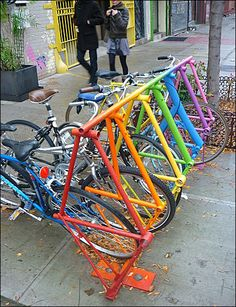
\includegraphics[scale=0.6]{rainbow-bikeshed.jpg}
\end{frame}

\begin{frame}
	\frametitle{Packaging base?}
	\pause
	\colorbox{red}{\makebox[\textwidth]{\textcolor{white}{Do not split}}}
	\pause
	\colorbox{orange}{\makebox[\textwidth]{Allow minimal installation}}
	\pause
	\colorbox{yellow}{\makebox[\textwidth]{No toolchain}}
	\pause
	\colorbox{green}{\makebox[\textwidth]{No sendmail}}
	\pause
	\colorbox{blue}{\makebox[\textwidth]{\textcolor{white}{No development file}}}
	\pause
	\colorbox{indigo!75}{\makebox[\textwidth]{\textcolor{white}{No documentation}}}
	\pause
	\colorbox{violet}{\makebox[\textwidth]{\textcolor{white}{I want debug files}}}
\end{frame}

\begin{frame}
	\frametitle{Let's try to paint it rainbow}
	\colorbox{red}{\makebox[\textwidth]{\textcolor{white}{FreeBSD FreeBSD-base FreeBSD-kernel FreeBSD-docs}}}
	\pause
	\colorbox{orange}{\makebox[\textwidth]{FreeBSD-minimal FreeBSD-develepment}}
	\pause
	\colorbox{yellow}{\makebox[\textwidth]{FreeBSD-toolchain}}
	\pause
	\colorbox{green}{\makebox[\textwidth]{FreeBSD-sendmail FreeBSD-openssl FreeBSD-bhyve}}
	\pause
	\colorbox{blue}{\makebox[\textwidth]{\textcolor{white}{runtime separated from development files}}}
	\pause
	\colorbox{indigo!75}{\makebox[\textwidth]{\textcolor{white}{FreeBSD-docs (does not concern manpages)}}}
	\pause
	\colorbox{violet}{\makebox[\textwidth]{\textcolor{white}{-debug packages}}}
\end{frame}

\begin{frame}
	\frametitle{Why?}
	\begin{itemize}
		\item Binary upgrade of the system
			\begin{itemize}
				\item For RELEASE (like freebsd-update)
				\item For STABLE
				\item For CURRENT
			\end{itemize}
		\item Allow users to do fine grain installations (no toolchain, no sendmail, etc.)
		\item Allow developers to provide packages for users to test
		\item Fine grain merging of configuration files
		\item Being able to upgrade the loader and its configurations!
	\end{itemize}
\end{frame}

\begin{frame}[fragile]
	\frametitle{Goals}
	\begin{itemize}
		\item Integrated into the build system
			\begin{lstlisting}
			$ make packages
			\end{lstlisting}
		\item Buildable as regular user
		\item Reproductible
			\begin{lstlisting}
			$ make repackages
			\end{lstlisting}
		\item Automatic version bump on the right packages when patching
			a release
			\begin{lstlisting}
			$ make rerelease
			\end{lstlisting}
		\item Automatically handling configuration files (merging)
		\item Cross installable
	\end{itemize}
\end{frame}

\begin{frame}
	\frametitle{Versionning}
	\begin{itemize}
		\item CURRENT: 12.s<date>
		\item STABLE: After 11.0-RELEASE and before 11.1-RELEASE: 11.1.s<date>
		\item RELEASE:
			\begin{itemize}
				\item ALPHA: 11.0.aX
				\item BETA: 11.0.bX
				\item RC: 11.0.pX (not r to not confuse with "release")
				\item RELEASE: 11.0
				\item Security fix: 11.0\_1
			\end{itemize}
	\end{itemize}
\end{frame}

\begin{frame}
	\frametitle{Modification needed in pkg(8)}
	\begin{itemize}
		\item Handling file flags immutable (added in pkg 1.5)
		\item Ability to handle configuration files and merge them (added in pkg 1.5)
			\begin{itemize}
				\item new keyword @config
				\item 3 way merge code from the fossil VCS
			\end{itemize}
		\item Better support for cross installation:
			\begin{itemize}
				\item pkg -r <rootdir> (added in pkg 1.5)
				\item scripts PKG\_ROOTDIR (added in pkg 1.5)
			\end{itemize}
	\end{itemize}
\end{frame}

\begin{frame}
	\frametitle{Hooking in the build system}
	\begin{itemize}
		\item Reuse the -DNO\_ROOT mechanism
		\item Add tags to the generated mtree to determine packages content
		\item New targets:
			\begin{itemize}
				\item stageworld
				\item stagekernel
				\item packages
			\end{itemize}
		\item Packages metadata
			\begin{itemize}
				\item UCL manifest
				\item release/pkg
			\end{itemize}
	\end{itemize}
\end{frame}

\begin{frame}[fragile]
	\frametitle{Issues with the build system: NO\_ROOT}
	\begin{itemize}
		\item mtree(8):
			In \underline{stdout}:
			\begin{lstlisting}
			===> share/examples (install)
			.:      user (0, 1001, not modified: Operation not permitted)
			lib32:  user (0, 1001, not modified: Operation not permitted)
			lib32/dtrace: 
			        user (0, 1001, not modified: Operation not permitted)
			lib32/i18n: 
			        user (0, 1001, not modified: Operation not permitted)
			\end{lstlisting}
		\item chflags(1) vs modes:
			\begin{lstlisting}
			chflags: /usr/obj/home/bapt/dev/src-trees/release-pkg/stage/usr/bin/chpass: Operation not permitted
			chflags: /usr/obj/home/bapt/dev/src-trees/release-pkg/stage/usr/bin/passwd: Operation not permitted
			\end{lstlisting}

		\item Installation not using install(1)
	\end{itemize}
\end{frame}

\begin{frame}[fragile]
	\frametitle{Issues with the build system: installworld crap}
	\begin{itemize}
		\item bsd.tests.mk/bsd.progs.mk installing files multiple times - BLOCKER
			\begin{lstlisting}
			===> Creating FreeBSD-runtime-11.0.s20150612175342
			pkg: duplicate file listing: /usr/tests/lib/libc/db/db_test, ignoring
			pkg: duplicate file listing: /usr/tests/lib/libc/gen/posix_spawn/h_nonexec, ignoring
			pkg: duplicate file listing: /usr/tests/lib/libc/gen/posix_spawn/h_zero, ignoring
			pkg: duplicate file listing: /usr/tests/lib/libc/gen/posix_spawn/h_nonexec, ignoring
			\end{lstlisting}
		\item etc configuration files
			\begin{itemize}
				\item{generates the db files}
				\item{not installed at installworld time}
			\end{itemize}
	\end{itemize}
\end{frame}

\begin{frame}[fragile]
	\frametitle{End user point of view}
	\begin{itemize}
		\item Upgrading the system:
			\begin{lstlisting}
			$ pkg upgrade
			\end{lstlisting}
		\item Creating a FreeBSD disk:
			\begin{lstlisting}
			$ mkdir newimage
			$ pkg -r newimage install FreeBSD
			$ makefs -B little FreeBSD.img newimage
			\end{lstlisting}
		\item Creating an armv6 disk image on an amd64 host:
			\begin{lstlisting}
			$ mkdir armv6image
			$ pkg -r armv6image -o "ABI=FreeBSD:11:armv6" install FreeBSD-minimal
			$ makefs -B little FreeBSD.img armv6newimage
			\end{lstlisting}
		\item Upgrading and armv6 image on an amd64 host:
			\begin{lstlisting}
			$ pkg -r armv6image upgrade
			\end{lstlisting}
	\end{itemize}
\end{frame}

\begin{frame}
	\frametitle{Questions?}
	\center
	\Huge Thanks
\end{frame}
\end{document}
